\section{Human Annotation Protocol}\label{apdx:annotation}
Our annotation process involves ten trained annotators with master’s degrees, who are recruited and compensated in compliance with local labor laws and regulations. Annotators are provided with clear written guidelines to ensure consistency and accuracy, as outlined in our annotation protocol (see Figures~\ref{fig:annotation-1} and~\ref{fig:annotation-2}). All tasks are designed to avoid sensitive personal data, and all annotated content is in English with no identifying information. 
The process includes task expansion—transforming generalized instructions into explicit, executable tasks—and strict result verification to minimize errors. Quality control measures include verification passes and clear formatting rules to improve annotation reliability. 
No annotator is exposed to harmful, discriminatory, or unsafe content during the process, and all work adheres to the Code of Ethics regarding fairness, privacy, and legal compliance.

\vspace{-10mm}
\begin{figure}[h!]
    \centering
    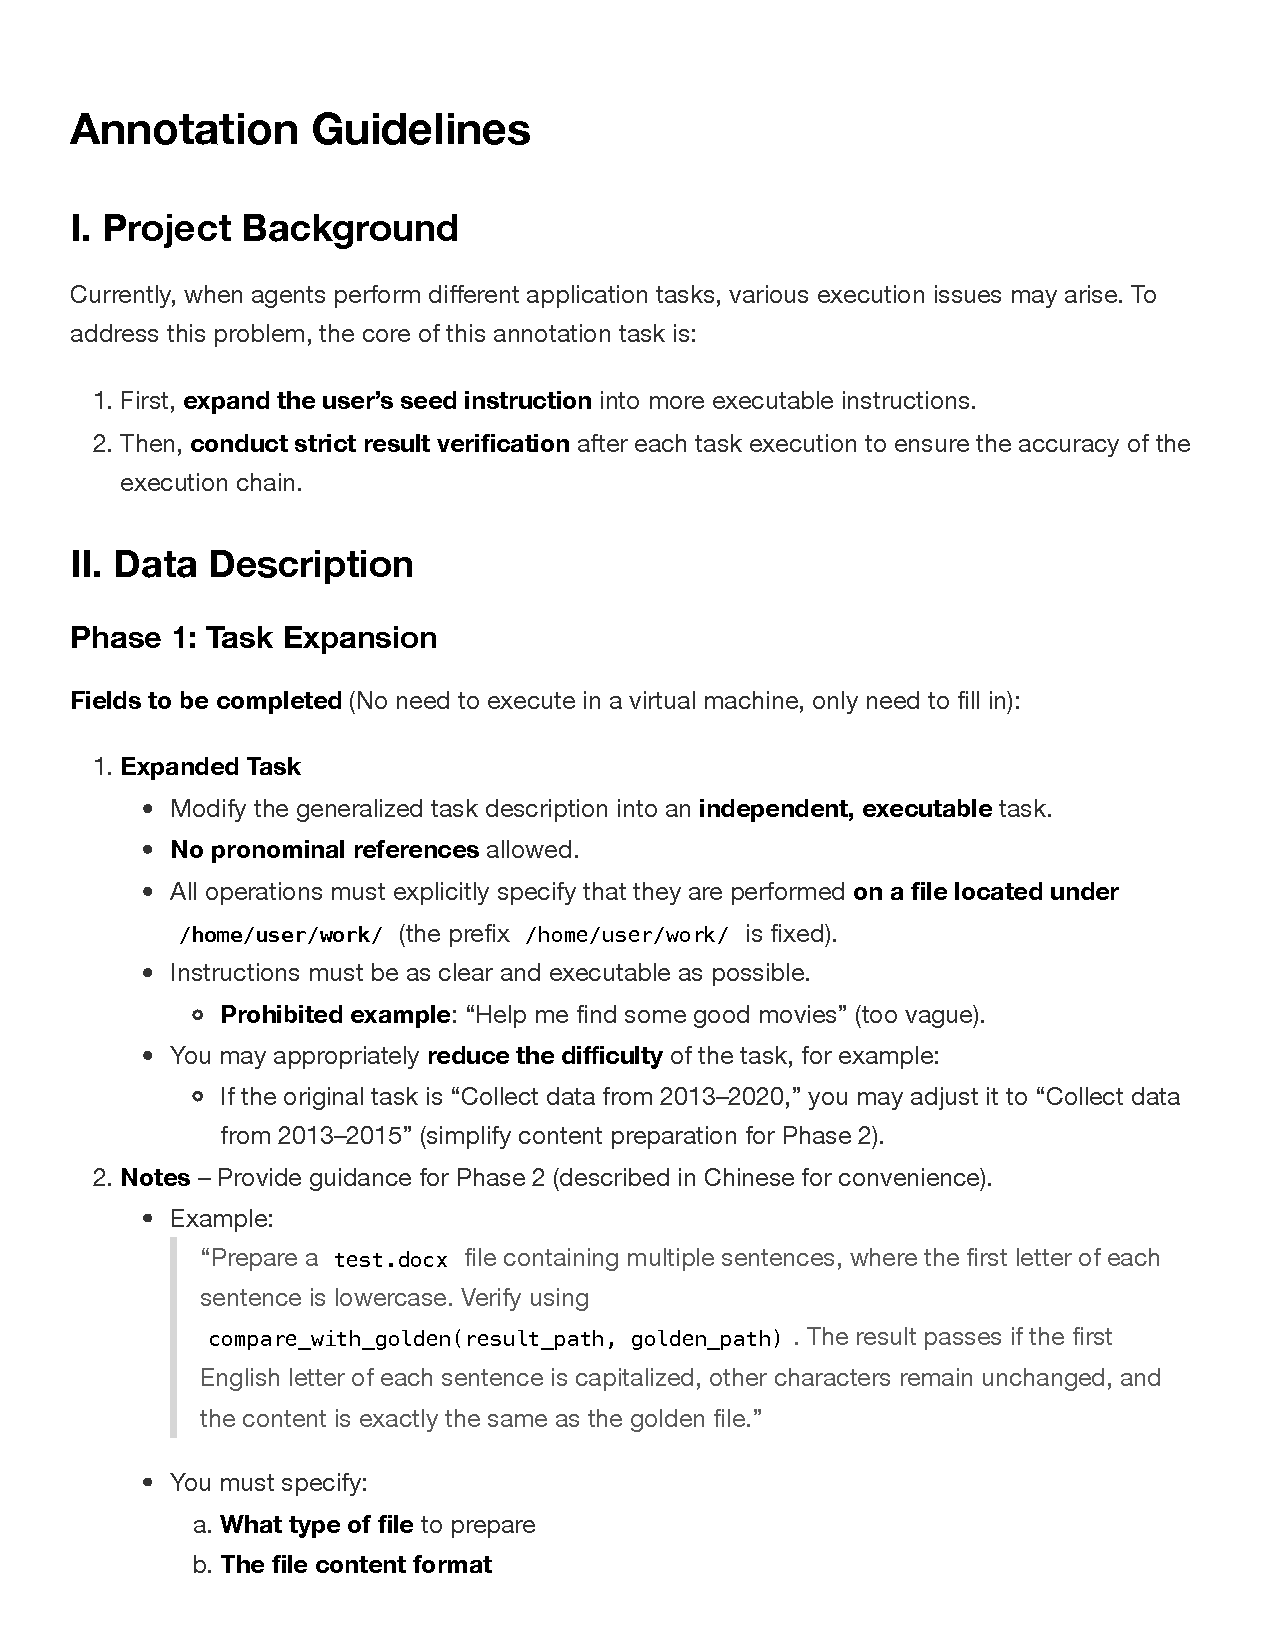
\includegraphics[width=\textwidth,height=\textheight,keepaspectratio]{images/annotation-1.pdf}
    \vspace{-3mm}
    \caption{Document for Human Annotation (1 / 2)}
    \label{fig:annotation-1}
\end{figure}

\begin{figure}[h!]
    \centering
    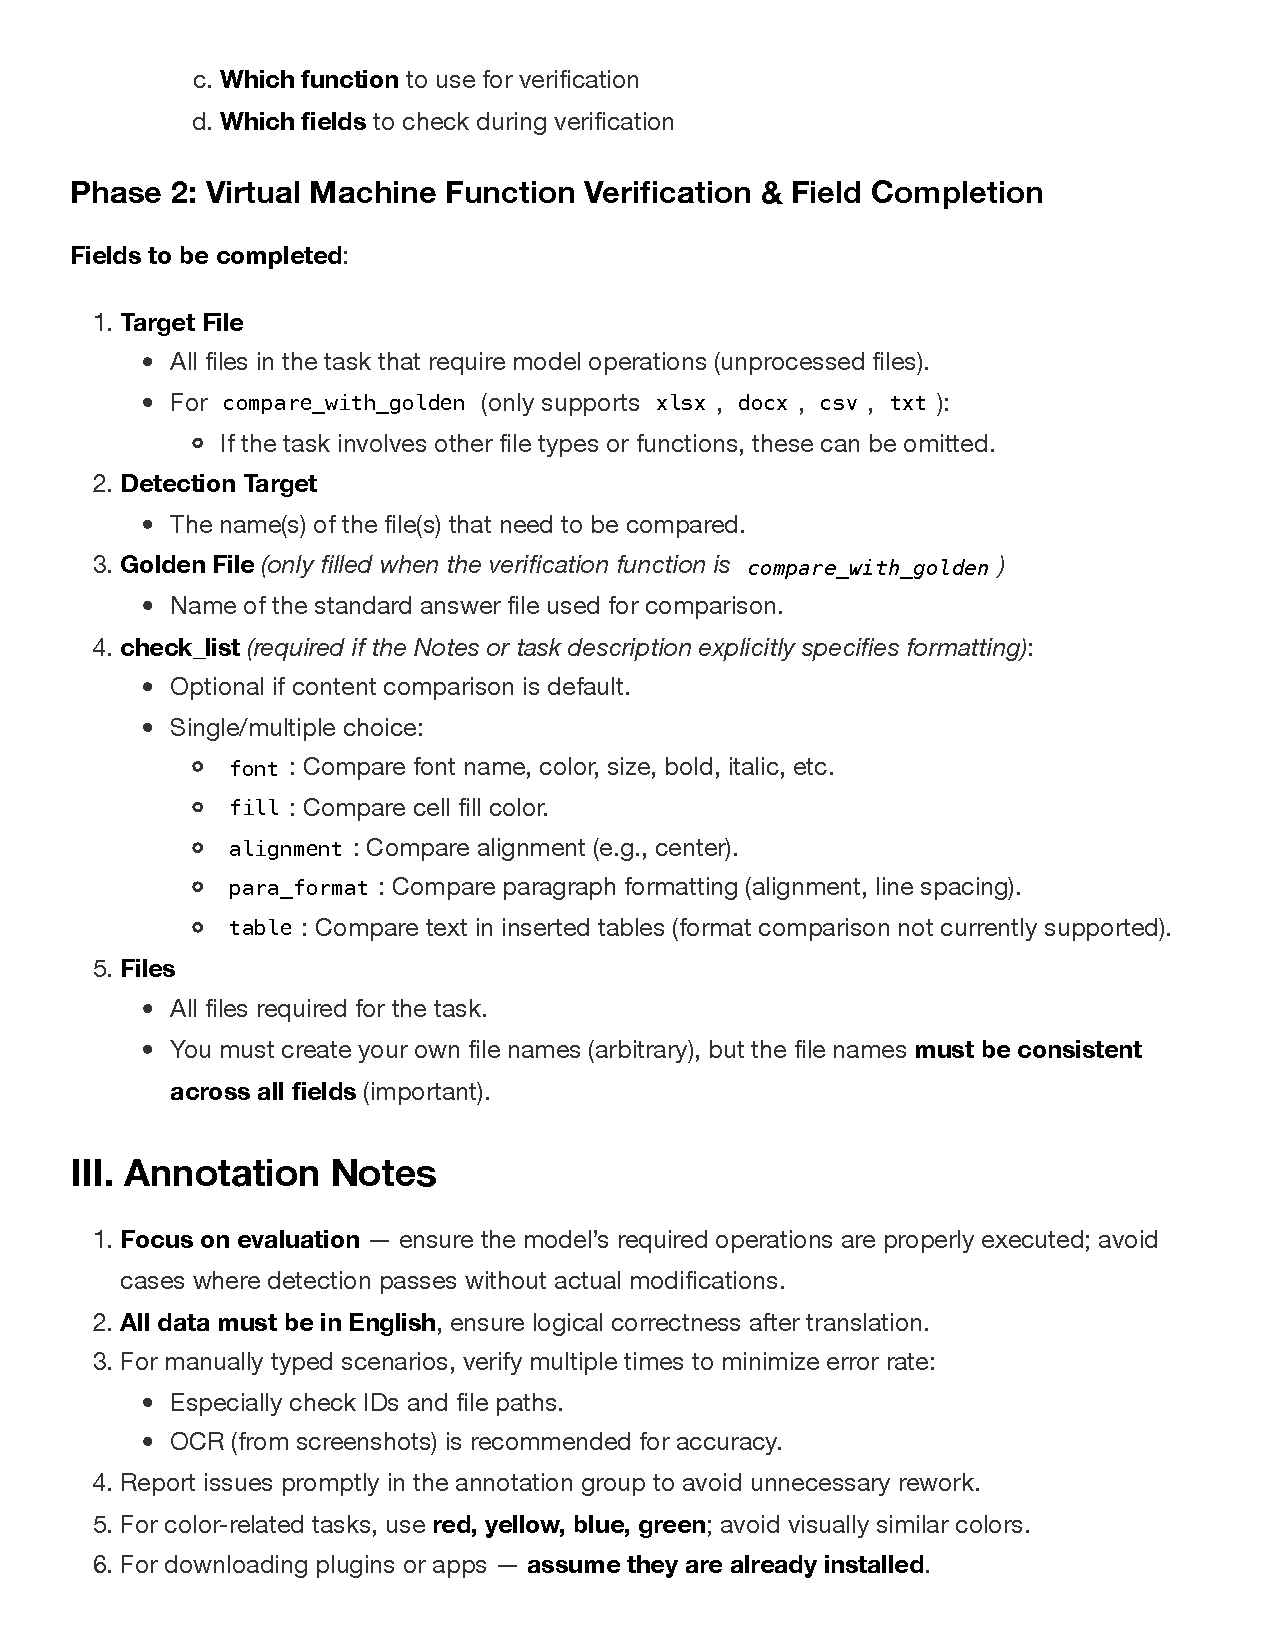
\includegraphics[width=\textwidth,height=\textheight,keepaspectratio]{images/annotation-2.pdf}
    \vspace{-3mm}
    \caption{Document for Human Annotation (2 / 2)}
    \label{fig:annotation-2}
\end{figure}

\clearpage